\section{Implications for the postmerger gravitational-wave peak}
\label{sec:gw}

The postmerger gravitational-wave spectrum of a neutron-star merger is dominated by a single peak at $f_{\rm peak}\approx2$--$4\,\kHz$, the fundamental quadrupolar ($m=2$) oscillation of the remnant \cite{Stergioulas:2011gd,Takami:2014tva}.
Simulations with a first-order transition to quark matter find that conversion of the core shifts $f_{\rm peak}$ by several hundred Hz relative to a purely hadronic remnant \cite{Bauswein:2018bma,Most:2018eaw,Weih:2019xvw,Bauswein:2020ggy,Fujimoto:2022xhv,Espino:2023llj}.
All of these simulations convert matter the instant its pressure exceeds $p_\text{crit}$, which is the instantaneous-conversion prescription described in the introduction.
Here we estimate how the finite boundary speed obtained in Sec.~\ref{sec:results} changes that prediction.
We write $f_{\rm peak}^{\infty}$ for the peak frequency under instantaneous conversion and $f_{\rm peak}^{\rm finite}$ for the peak frequency when conversion proceeds by boundary propagation at the calculated speed.

\textbf{Converted fraction behind a finite-speed front.}
At each time $t$, quark matter is thermodynamically favored in the region
\begin{equation}
\Omega_{\rm crit}(t)
=\left\{\boldsymbol{x}:\,P(\boldsymbol{x},t)>p_\text{crit}\right\},
\label{eq:critical_region}
\end{equation}
with $p_\text{crit}$ determined as in Sec.~\ref{sec:results}.
The instantaneous prescription converts all of $\Omega_{\rm crit}$ at every instant.
With a finite conversion speed, matter in $\Omega_{\rm crit}$ converts only after a phase boundary has swept over it, which we track with an indicator field $Y_q(\boldsymbol{x},t)$: $Y_q=1$ where matter has deconfined and $Y_q=0$ elsewhere.
Matter with $P>p_\text{crit}$ and $Y_q=0$ is the metastable nuclear matter whose conversion speed we calculated in Sec.~\ref{sec:speed}.
The indicator also encodes hysteresis: converted matter stays converted if the local pressure later falls back below $p_\text{crit}$.

The motion of the boundary in the merger frame follows from Sec.~\ref{sec:speed}.
The front advances into the nuclear matter at speed $u(0^-)$ relative to that matter, so the boundary moves with the local fluid velocity plus $u(0^-)$ along the boundary normal, directed into the nuclear phase.
The calculated speeds obey $u(0^-)\lesssim10^{-5}$ in natural units, so we do not distinguish between proper and ordinary velocity in this section.
Advection by the merger flow rearranges the boundary but converts no matter; the converted volume grows only through the normal propagation at $u(0^-)$.
In a simulation, $Y_q$ can be implemented as a marker (level-set) field transported with this velocity; Appendix~\ref{sec:finite_rate_implementation} gives the prescription.

We measure the progress of conversion by the converted volume fraction of the critical-pressure region,
\begin{equation}
X_q(t)
=\frac{1}{V_{\rm crit}(t)}
\int_{\Omega_{\rm crit}(t)}Y_q(\boldsymbol{x},t)\,dV\,,
\label{eq:converted_fraction}
\end{equation}
where $V_{\rm crit}(t)$ is the volume of $\Omega_{\rm crit}(t)$.
The same definition can be weighted by baryon density, or by the local sensitivity of the $m=2$ mode to the equation of state \AHcom{what does this mean?}\JScom{The index $m$ is the azimuthal mode number.
A perturbation of a nearly axisymmetric remnant can be expanded in the angle $\phi$ about the rotation axis into terms that vary as $e^{i(m\phi-\omega t)}$, and $m$ counts how many full cycles the pattern completes in one turn around that axis.
An $m=0$ pattern is axisymmetric, a breathing or quasi-radial motion; $m=1$ is a one-sided displacement; $m=2$ stretches the equatorial cross-section into a rotating bar.
Only the bar radiates appreciably.
Gravitational-wave emission has no monopole or dipole part, so it comes from the mass quadrupole, and within the quadrupole the $m=2$ component has a time-varying moment while the $m=0$ (axisymmetric) component does not.
Strictly, $m$ fixes only the azimuthal shape: the dominant peak is the $\ell=m=2$ fundamental mode, with smaller $m=2$ contributions from higher multipoles $\ell=3,4,\dots$
A pattern $\propto e^{i(2\phi-\omega t)}$ rotates rigidly at angular speed $\omega/2$ and looks the same after half a turn, so a distant observer sees the quadrupole repeat twice per revolution and the wave emerges at $f_{\rm peak}=\omega/2\pi$.}, without changing the estimates below.

Evaluating $X_q$ requires a geometry for $\Omega_{\rm crit}$.
During the first milliseconds the critical-pressure region follows the rotating double-core pattern: in the equatorial plane $\Omega_{\rm crit}$ consists of two congruent lobes that wrap around one another, a taiji (yin--yang) shape with one pressure maximum in each lobe.
This is the same $m=2$ deformation that carries the mass quadrupole responsible for the postmerger emission, so the converted fraction and its mode-weighted variant refer to the same region.
The pattern corotates with the fluid cores, so rotation advects the lobes and, as noted above, converts no matter.
Conversion starts from a seed at each pressure maximum, and over the postmerger emission window $\Delta t_{\rm pm}$ the two converted regions grow as spheres of radius $u(0^-)\,\Delta t_{\rm pm}$ until they span their lobes, so
\begin{equation}
X_q
=\min\!\left\{1,\,
\left[\frac{u(0^-)\,\Delta t_{\rm pm}}{R_{\rm lobe}}\right]^{3}
\right\},
\label{eq:lobe_fraction}
\end{equation}
where $R_{\rm lobe}\equiv[3V_{\rm crit}/(8\pi)]^{1/3}$ is the effective radius of one lobe and $V_{\rm crit}$ the total volume of $\Omega_{\rm crit}$.

\textbf{Catch-up within the emission window.}
The finite-rate remnant matches the instantaneous-conversion remnant during the epoch when $f_{\rm peak}$ is accumulated only if the front reaches every point of $\Omega_{\rm crit}$ within that window:
\begin{equation}
u(0^-)\gtrsim\frac{L_{\rm max}}{\Delta t_{\rm pm}}
\quad\Longrightarrow\quad
f_{\rm peak}^{\rm finite}\simeq f_{\rm peak}^{\infty}\,,
\label{eq:catch_up}
\end{equation}
where $L_{\rm max}$ is the largest propagation distance, measured through the matter, from the initial seed surface to any point of $\Omega_{\rm crit}$.

Both sides of Eq.~\eqref{eq:catch_up} are fixed by known numbers.
Quark cores in instantaneous-conversion simulations extend over a few kilometers \cite{Most:2018eaw,Bauswein:2018bma}, so the lobes have effective radii $R_{\rm lobe}\approx0.7$--$2\,\km$, and the postmerger peak is accumulated over $\Delta t_{\rm pm}\approx5$--$20\,\text{ms}$ of emission \cite{Takami:2014tva,Vretinaris:2019spn}.
The seed sits at the head of its lobe and the farthest matter at the tip of the wrapping tail, so $L_{\rm max}\approx2R_{\rm lobe}$ and catching up requires $u(0^-)\gtrsim10^{5}$--$10^{6}\,\m\,\s^{-1}$.
The maximum boundary speeds of Sec.~\ref{sec:results} at merger temperatures, $u_{\rm max}(0^-)\approx10^{2}$--$10^{3}\,\m\,\s^{-1}$, fall short by two to four orders of magnitude.
This is the quantitative form of the concern raised in the introduction: the instantaneous prescription implicitly assumes boundary speeds near $10^{6}\,\m\,\s^{-1}$, while weak-interaction-limited propagation reaches at most $10^{3}\,\m\,\s^{-1}$.
The converted fraction is then negligible.
For $u(0^-)=10^{3}\,\m\,\s^{-1}$ and $\Delta t_{\rm pm}=10\,\text{ms}$ each front sweeps only $10\,\m$, and Eq.~\eqref{eq:lobe_fraction} with $V_{\rm crit}=3\,\km^{3}$ ($R_{\rm lobe}\approx0.7\,\km$) gives $X_q\approx3\times10^{-6}$.

On the timescale of the postmerger emission, weak-interaction-limited conversion is frozen: the phase boundary is a comoving surface and $\Omega_{\rm crit}$ stays filled with metastable nuclear matter.
Interface-mode analyses of the inspiral assume the same frozen composition \cite{Tonetto:2020bie,Counsell:2025hcv,Pereira:2025xsi}; here it follows from the microphysics under merger conditions.
Converting the whole core within the window would instead need seeds spread through the volume, spaced by no more than $\sim2\,u_{\rm max}(0^-)\,\Delta t_{\rm pm}\approx20\,\m$.
Whether nucleation can supply that seed density is a question of bubble-nucleation physics rather than boundary propagation, and we do not address it here.
Hydrodynamic instabilities of the front could also raise the effective conversion rate above our planar bound, as discussed in Sec.~\ref{sec:conclusion}.

\textbf{Peak-frequency shift and observability.}
Let $\Delta f_{\rm PT}$ denote the signed shift of the peak frequency between a remnant whose critical-pressure region is fully converted and one in which it stays (metastable) nuclear matter.
This is an equilibrium quantity, fixed by the equation of state.
It can be calibrated from instantaneous-conversion simulations, which find $|\Delta f_{\rm PT}|$ of several hundred Hz for strong transitions \cite{Bauswein:2018bma,Most:2018eaw,Weih:2019xvw}.
It can also be read off observationally, as a deviation of $f_{\rm peak}$ from hadronic empirical relations of the form $f_{\rm peak}^{\infty}=F(\mathcal{M}_{\rm chirp},R_{1.8})$, where $\mathcal{M}_{\rm chirp}$ is the chirp mass and $R_{1.8}$ the radius of a cold, nonrotating $1.8\,M_\odot$ star \cite{Bauswein:2012ya,Vretinaris:2019spn}.
The two prescriptions differ only in the unconverted part of $\Omega_{\rm crit}$, so to leading order in that volume the peak frequency interpolates linearly in the converted fraction,
\begin{equation}
f_{\rm peak}^{\rm finite}
\simeq
f_{\rm peak}^{\infty}
-\bigl[1-X_q(\Delta t_{\rm pm})\bigr]\,
\Delta f_{\rm PT}
\label{eq:finite_peak_frequency}
\end{equation}
and the discrepancy between the prescriptions is
\begin{equation}
\Delta f_{\rm peak}
\equiv
f_{\rm peak}^{\infty}-f_{\rm peak}^{\rm finite}
\simeq
\bigl[1-X_q\bigr]\,\Delta f_{\rm PT}\,.
\label{eq:rate_shift}
\end{equation}
For $X_q\to1$ this reduces to the instantaneous result; for $X_q\to0$ the remnant rings at the frequency of the unconverted, metastable core.

Figure~\ref{fig:rate_deficit} shows $\Delta f_{\rm peak}$ as a function of the boundary speed, for seven values of $\Delta f_{\rm PT}$ calibrated as endpoint differences from published instantaneous-conversion simulations \cite{Prakash:2023afe,Bauswein:2018bma}.
At the calculated $u_{\rm max}(0^-)\approx10^{2}$--$10^{3}\,\m\,\s^{-1}$ the suppression factor is $1-X_q\geq0.9999$, so the transition leaves almost no imprint on the peak: $f_{\rm peak}^{\rm finite}\simeq f_{\rm peak}^{\infty}-\Delta f_{\rm PT}$, and the shift predicted by instantaneous-conversion simulations is not realized.
Put differently, the instantaneous prescription overestimates the converted volume by a factor of order $10^{5}$ and misplaces the peak by the full $|\Delta f_{\rm PT}|$.

\begin{figure}[t]
  \centering
  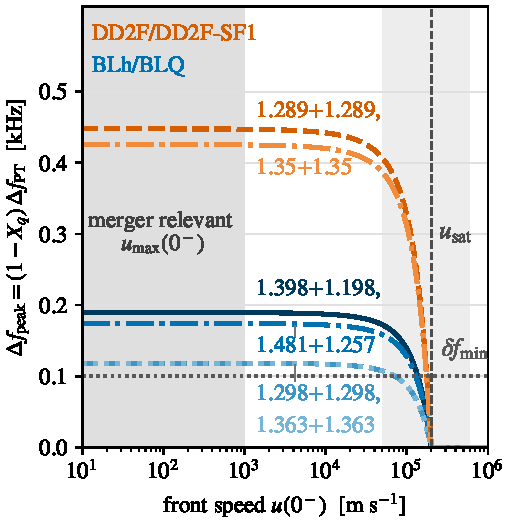
\includegraphics[width=\columnwidth]{Plots/f_peak.pdf}%
  \caption{Finite-rate frequency deficit $\Delta f_{\rm peak}=(1-X_q)\,\Delta f_{\rm PT}$ from Eqs.~\eqref{eq:lobe_fraction} and \eqref{eq:rate_shift}, using the two-lobed geometry with $R_{\rm lobe}=0.7\,\km$ and $\Delta t_{\rm pm}=10\,\text{ms}$.
  Each curve uses a $\Delta f_{\rm PT}$ calibrated as the endpoint difference between hybrid-EOS and purely hadronic instantaneous-conversion simulations, labeled by EOS pair and binary masses \cite{Prakash:2023afe,Bauswein:2018bma}; the two BLh/BLQ binaries with $\Delta f_{\rm PT}=0.123\,\kHz$ overlap.
  The shaded band marks the maximum boundary speeds calculated in Sec.~\ref{sec:results} at merger temperatures; the dashed line is the geometric saturation speed $u_{\rm sat}=R_{\rm lobe}/\Delta t_{\rm pm}$ above which the front would convert the whole region within the emission window.
  Throughout the shaded band the deficit equals the full $\Delta f_{\rm PT}=0.12$--$0.78\,\kHz$, above the $\delta f_{\rm min}\approx0.1\,\kHz$ resolution expected for next-generation postmerger detections \cite{Clark:2015zxa,Breschi:2022ens}.}
  \label{fig:rate_deficit}
\end{figure}

Whether this is detectable depends on the frequency resolution of postmerger observations.
The discrepancy is measurable if
\begin{equation}
\bigl[1-X_q\bigr]\,\bigl|\Delta f_{\rm PT}\bigr|
\gtrsim\delta f_{\rm min}\,,
\label{eq:observability}
\end{equation}
where $\delta f_{\rm min}$ is the smallest resolvable shift of the peak.
Next-generation detectors are expected to reach $\delta f_{\rm min}\approx10^{2}\,\text{Hz}$ at postmerger signal-to-noise ratio ${\sim}10$ \cite{Clark:2015zxa,Breschi:2022ens}, and Bayesian recoveries can distinguish phase-transition-induced deviations of this size \cite{Prakash:2023afe}.
The calibrated $|\Delta f_{\rm PT}|$ span $0.12$--$0.78\,\kHz$ (Fig.~\ref{fig:rate_deficit}) and $1-X_q\simeq1$, so Eq.~\eqref{eq:observability} holds for every case.
A detected postmerger peak from a remnant that crosses the transition should therefore sit at the metastable hadronic value rather than at the shifted equilibrium value, unless nucleation seeds conversion densely enough to bypass the front-speed bound.

The inputs to this estimate (the geometry of $\Omega_{\rm crit}$, the emission window $\Delta t_{\rm pm}$, and the calibration $\Delta f_{\rm PT}$) all depend on the binary chirp mass, so Eqs.~\eqref{eq:finite_peak_frequency} and \eqref{eq:observability} define $f_{\rm peak}^{\rm finite}(\mathcal{M}_{\rm chirp},u(0^-))$ once those inputs come from equilibrium sequences or from numerical relativity.
We do not predict the strain amplitude of the peak; that requires the excitation energy and damping of the $m=2$ mode in addition to its frequency.

